\documentclass[10pt,a4paper]{article}

%\documentclass[10pt,onecolumn,letterpaper]{IEEEtran}

\usepackage{setspace}
%\AtBeginDocument{\setstretch{.9}}
%\doublespacing  % doublespacing is done after title and before abstract

\usepackage{caption}
\usepackage{subcaption}
% \usepackage[title]{appendix}

%\usepackage[margin=0.25in]{geometry}

%\usepackage{lineno}
%\linenumbers

\usepackage{fullpage}
\usepackage{authblk}
\usepackage[utf8]{inputenc}
\usepackage{amsmath,bm}
\usepackage{amsthm}
\usepackage{amssymb}
\usepackage{hyperref}
\usepackage{adjustbox}
\usepackage{multirow}
\usepackage{graphicx}
\usepackage{booktabs}
\usepackage{caption}
\usepackage{subcaption}
\usepackage[table]{xcolor}
\usepackage{tabu}
\usepackage{subcaption}
\usepackage{longtable}
\usepackage{amssymb}
\usepackage{footnote}
\usepackage{hyperref}
\usepackage{multirow}
\usepackage{comment}
\usepackage{cite}
\usepackage{threeparttable}
\usepackage{makecell}
\usepackage{mathtools} % for multiline-multicase equation
\usepackage{float}
\usepackage{array}
\usepackage{tabularx} % in the preamble
\usepackage{tikz}
\usepackage{ulem}
\usepackage{algorithm2e}
\usepackage{pifont}

\usepackage{tabularx}
\newcolumntype{Y}{>{\centering\arraybackslash}X}
\newcolumntype{C}[1]{>{\centering\arraybackslash}m{#1}}

% \usepackage[demo]{graphicx}
% \usepackage[utf8]{inputenc}
% \usepackage{subfigure}
\usepackage{xcolor}
\newcommand{\add}[1]{{\color{blue} #1}}
\newcommand{\addb}[1]{{\color{red} #1}}
\newcommand{\SR}[1]{{\color{red} #1}}
\newcommand{\methodname}{{\color{purple}Method\_Name~}}

\newtheorem{theorem}{Theorem}[section]
\newtheorem{corollary}{Corollary}[theorem]
\newtheorem{lemma}[theorem]{Lemma}

% \renewcommand{\thetheorem}{\arabic{theorem}}
\renewcommand{\thefigure}{S\arabic{figure}}
\renewcommand{\thetable}{S\arabic{table}}
\renewcommand{\theequation}{S\arabic{equation}}

%\usepackage{booktabs, caption, makecell}
%\renewcommand\theadfont{\bfseries}
\usepackage{subfiles} % For subfiles
\usepackage{hyperref}
\usepackage[labelfont=bf]{caption}

\usepackage{xcolor}
\usepackage{xr}
\externaldocument[journal-]{journal-version}

\renewcommand\theadalign{bc}
\renewcommand\theadfont{\bfseries}
\renewcommand\theadgape{\Gape[4pt]}
\renewcommand\cellgape{\Gape[4pt]}



\makesavenoteenv{tabular}
\makesavenoteenv{table}

\hypersetup{
    urlcolor=blue,
}

\title{Supplementary material for \\ Correcting quartet distribution improves phylogenomic analyses despite gene tree estimation error
\author[1,*]{Navid Bin Hasan$^{1}$, Sohaib$^{1}$, and Md. Shamsuzzoha Bayzid}
}
\affil[1]{Department of Computer Science and Engineering\protect \\
Bangladesh University of Engineering and Technology, Dhaka-1205, Bangladesh}
% \affil[2]{Department of Computer Science\protect\\University of Maryland, College Park, Maryland 20742, USA}
%\affil[3]{Department of Computer Science and Engineering\protect\\The Ohio State University, Ohio 43210, USA}
%\affil[$\dag$]{These authors contributed equally to this work}
\affil[*]{Corresponding author: shams\_bayzid@cse.buet.ac.bd}
\date{}

\begin{document}
\maketitle

These supplementary materials present additional results, supplementary figures, and tables.

% \section{Additional Results}
% \clearpage

% \section{QT-WEAVER: pseudo-code}
% \label{app:pseudocode}

% % \RestyleAlgo{ruled}

\normalem %%%% disable auto underline

\SetKwComment{Comment}{/* }{ */}
\IncMargin{1em}

\begin{algorithm}
\SetKwData{Left}{left}\SetKwData{This}{this}\SetKwData{Up}{up}
\SetKwFunction{Union}{Union}\SetKwFunction{FindCompress}{FindCompress}
\SetKwInOut{Input}{Input}\SetKwInOut{Output}{Output}

\Input{$\mathcal{QD_E}$, set of weighted quartets \\ 
$S$, set of all taxa
}
\Output{$\mathcal{QD'_E}$, set of weighted quartets with adjusted weights}
\BlankLine

\Comment{$\mathcal{A} $ is the set of adjusted quartets}
$\mathcal{A} \leftarrow \emptyset$; 

\ForEach{$q \in \mathcal{QD_E}$ }{
    

    \If(\tcp*[h]{already adjusted} ){$q \in \mathcal{A}$}{\label{lt}
            continue
    }
    
    \Comment{ Generate all 3 quartets on the leaves of $q$}
    $\mathcal{T} \leftarrow $ GenerateQuartets($L(q)$) \\

   
    $s \leftarrow 0$ \tcp{sum of actual weights of quartets in $\mathcal{T}$} \\
    $s' \leftarrow 0$ \tcp{sum of adjusted weights of quartets in $\mathcal{T}$}\\
    
    \ForEach{ $q_i \in \mathcal{T}$ }{\label{forins}

        $C_i \leftarrow 0$ \tcp{Conflict score of $q_i$}

        $s \leftarrow s + W_i$
        
        $Z_i \leftarrow $ \emptyset $ \;
        \ForEach{ $ t \in S \setminus L(q_i) $ }{ \label{forins}
            \Comment{For each external taxa, we generate 28 conflict pairs}
            $Z_i \leftarrow Z_i \cup $ GenerateConflicts($q_i, t$)
        }

        \ForEach{ $ (q_j, q_k) \in Z_i $ }{  \label{forins}
            \If(\tcp*[h]{Using Product of Weights definition} ){ heuristic is PoW }{\label{lt}
                $C_i \leftarrow C_i + W_j \cdot W_k$
            }
            \ElseIf(\tcp*[h]{Using Minimum of Weights definition} ){ heuristic is MoW } {
                $C_i \leftarrow C_i + min( W_j , W_k )$
            }
            
        }

        $ W_i' \leftarrow \frac{W_i}{C_i} $ \\
        $ s' \leftarrow s' + W_i'$
        
    }

    \Comment{Normalize the weights}
    \ForEach{ $q_i \in \mathcal{T}$ }{\label{forins}
        $W_i' \leftarrow \frac{s}{s'} \cdot W_i' $
    }

     $ \mathcal{A} \leftarrow \mathcal{A} \cup \mathcal{T} $ \\
    
    % \lForEach{element $e$ of the line $i$}{ \label{forins}
    % \FindCompress{p}
    % }
}
\caption{QT-WEAVER}\label{qtweaver-algo}
\end{algorithm}

\DecMargin{1em}
\ULforem %%%% enable auto underline

% \RestyleAlgo{ruled}

% \normalem %%%% disable auto underline

% \SetKwComment{Comment}{/* }{ */}
% \IncMargin{1em}

% \begin{algorithm}
% \SetKwData{Left}{left}\SetKwData{This}{this}\SetKwData{Up}{up}
% \SetKwFunction{Union}{Union}\SetKwFunction{FindCompress}{FindCompress}
% \SetKwInOut{Input}{Input}\SetKwInOut{Output}{Output}

% \Input{$\mathcal{QD_E}$, set of weighted quartets \\ 
% $S$, set of all taxa
% }
% \Output{$\mathcal{QD'_E}$, set of weighted quartets with adjusted weights}
% \BlankLine

% \Comment{$\mathcal{A} $ is the set of adjusted quartets}
% $\mathcal{A} \leftarrow \emptyset$; 

% \ForEach{$q \in \mathcal{QD_E}$ }{
    

%     \If(\tcp*[h]{already adjusted} ){$q \in \mathcal{A}$}{\label{lt}
%             continue
%     }
    
%     \Comment{ Generate all 3 quartets on the leaves of $q$}
%     $\mathcal{T} \leftarrow $ GenerateQuartets($L(q)$) \\

   
%     $s \leftarrow 0$ \tcp{sum of actual weights of quartets in $\mathcal{T}$} \\
%     $s' \leftarrow 0$ \tcp{sum of adjusted weights of quartets in $\mathcal{T}$}\\
    
%     \ForEach{ $q_i \in \mathcal{T}$ }{\label{forins}

%         $C_i \leftarrow 0$ \tcp{Conflict score of $q_i$}

%         $s \leftarrow s + W_i$
        
%         $Z_i \leftarrow $ \emptyset $ \;
%         \ForEach{ $ t \in S \setminus L(q_i) $ }{ \label{forins}
%             \Comment{For each external taxa, we generate 28 conflict pairs}
%             $Z_i \leftarrow Z_i \cup $ GenerateConflicts($q_i, t$)
%         }

%         \ForEach{ $ (q_j, q_k) \in Z_i $ }{  \label{forins}
%             \If(\tcp*[h]{Using Product of Weights definition} ){ heuristic is PoW }{\label{lt}
%                 $C_i \leftarrow C_i + W_j \cdot W_k$
%             }
%             \ElseIf(\tcp*[h]{Using Minimum of Weights definition} ){ heuristic is MoW } {
%                 $C_i \leftarrow C_i + min( W_j , W_k )$
%             }
            
%         }

%         $ W_i' \leftarrow \frac{W_i}{C_i} $ \\
%         $ s' \leftarrow s' + W_i'$
        
%     }

%     \Comment{Normalize the weights}
%     \ForEach{ $q_i \in \mathcal{T}$ }{\label{forins}
%         $W_i' \leftarrow \frac{s}{s'} \cdot W_i' $
%     }

%      $ \mathcal{A} \leftarrow \mathcal{A} \cup \mathcal{T} $ \\
    
%     % \lForEach{element $e$ of the line $i$}{ \label{forins}
%     % \FindCompress{p}
%     % }
% }
% \caption{QT-WEAVER}\label{qtweaver-algo}
% \end{algorithm}

% \DecMargin{1em}
% \ULforem %%%% enable auto underline


\section{QT-WEAVER configurations}
\label{app:configurations}

%As discussed in the methodology section, we will consider both the ``regular"  and the ``minimum" weighting schemes of QT-WEAVER for updating quartet weights. Additionally, apart from utilizing all 28 conflicting sets that a quartet $q$ belongs to for each taxon $e \notin L(q)$, we will also consider subsets of the set of 28 conflicting sets. We have analyzed subsets of sizes four, six, and eight in this study.

The comparison of the eight configurations of QT-WEAVER (the two weighting schemes combined with four different conflicting subsets) along with wQFM on the original distribution has been presented in Figure \ref{fig:rf_15_taxon_schemes}. The original distribution is derived by taking the frequency of each quartet in all gene trees (GTF: Gene Tree Frequency). We vary both the number of genes (100 and 1000) and the amount of gene tree estimation errors (by varying the sequence lengths from 100bp to 1000bp). As expected, the performance of the methods improves when the number of genes increases or when the gene tree estimation errors decrease. 
The MoW-based weighting scheme outperforms the PoW variant. Furthermore, subsets of four or six conflicting sets tend to perform better than all conflicting sets.

\begin{figure}[htbp]
    \centering 
    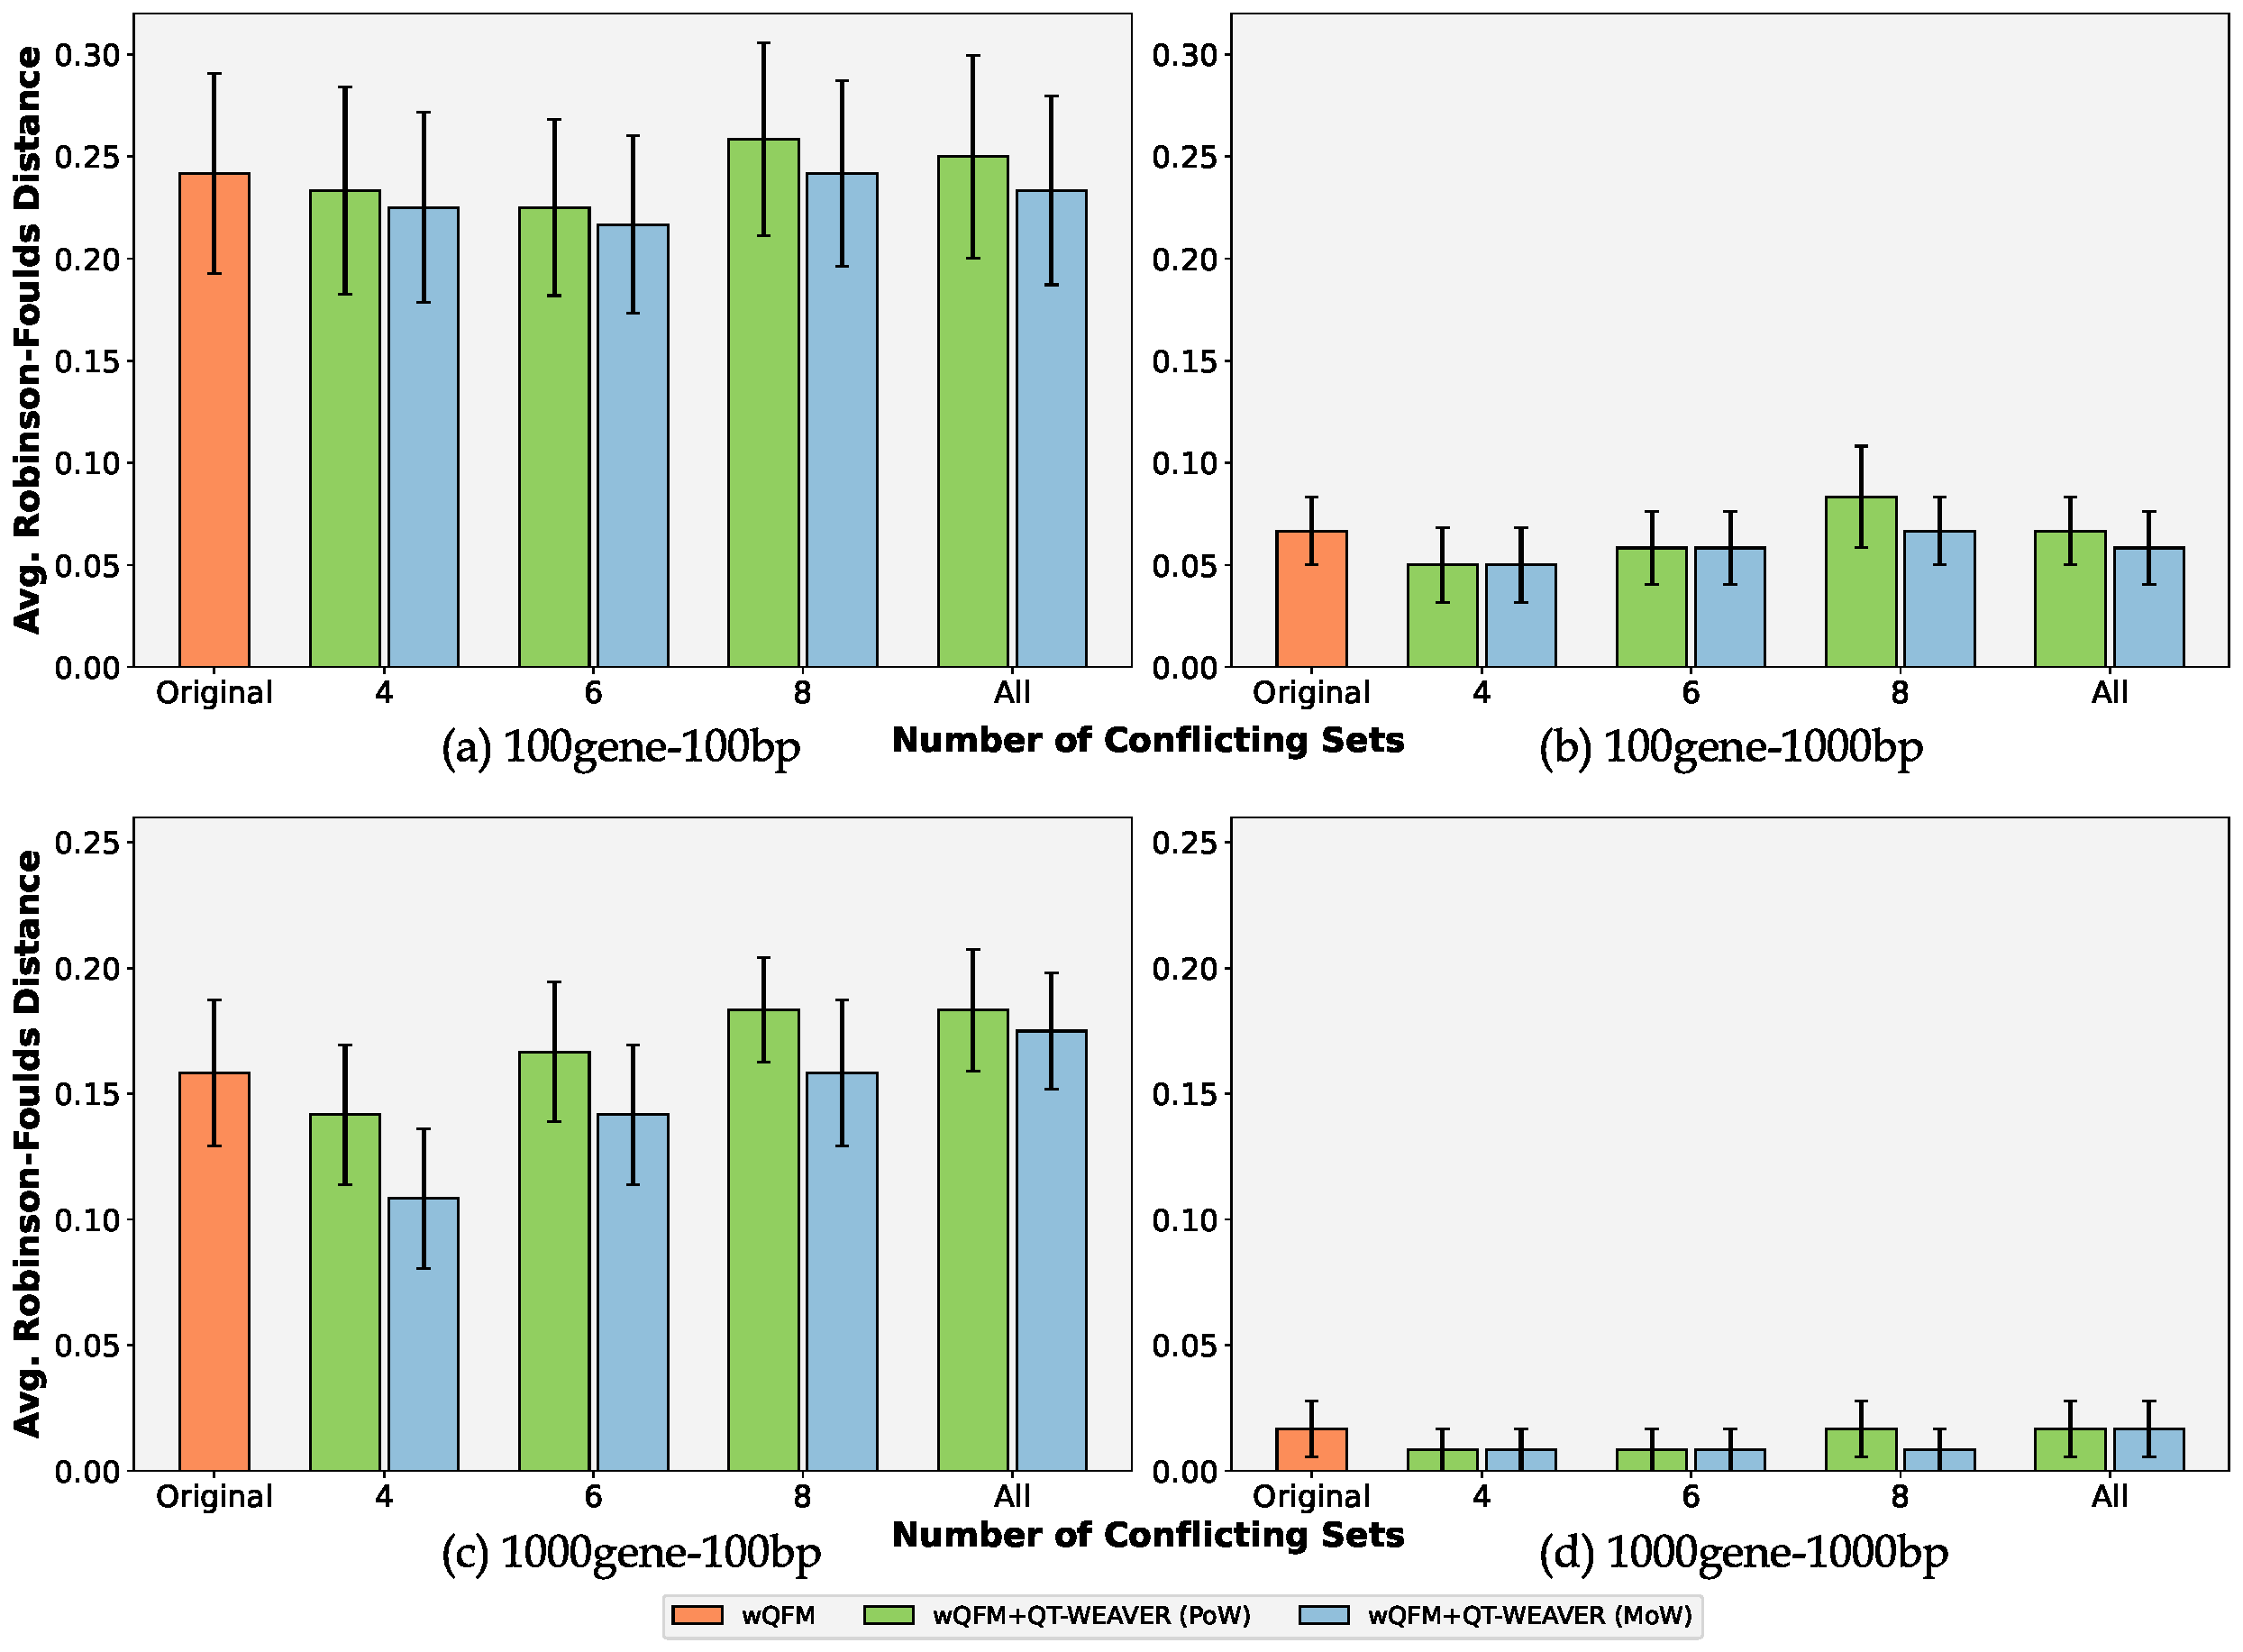
\includegraphics[width=.95\linewidth]{figures_new/1_15_modes.pdf}
    \caption{\textbf{Results on 15-taxon dataset.} Comparison of performance after correcting the weighted distributions using four, six, eight, and all 28 conflicting sets. We report the RF rates averaged over 10 replicates with standard errors. The distributions were amalgamated using wQFM. We show the effects of using both PoW and MoW weighting schemes. }
    \label{fig:rf_15_taxon_schemes}
\end{figure}

These results raise the question -- why does considering a small subset of all conflicting sets tend to yield better results? We hypothesize that using all 28 conflicting sets may impose excessive topological constraints on a quartet, making it challenging for QT-WEAVER to effectively distinguish among different topological variants.

In contrast, the six selected conflicting sets (as listed in Table \ref{table:conflicttable_six}) appear suitable for assessing conflict levels across quartet topologies, as indicated by our experimental results. While this specific choice of six sets lacks theoretical backing, we anticipate that the optimal subset--both in size and composition--may vary by dataset. Thus, an important research avenue involves automating the selection of these subsets, tailored to the topological features of the input gene trees, to optimize performance.

\begin{table}[h!]
\caption{We list the six conflicting sets chosen from all the conflicting sets in Table \ref{journal-table:conflicttable} from the main paper.}
    \centering
     \renewcommand{\arraystretch}{1.2}
    \begin{tabular}{|c|c|}
        \hline
        \textbf{Canonical Pair} & \textbf{Conflicting Quartets} \\ \hline

        $ab|cd$ \& $ac|be$ 
        & $ab|de$ $||$ $ae|bd$\\ \hline

        $ab|cd$ \& $ae|bc$ 
        & $ad|be$\\ \hline

        $ab|cd$ \& $ac|de$ 
        & $bd|ce$ $||$ $be|cd$\\ \hline

        $ab|cd$ \& $ad|ce$ 
        & $bc|de$\\ \hline
        
    \end{tabular}
    \label{table:conflicttable_six}
\end{table}

%So, why is it that only considering a small subset of all conflicting sets tends to yield better results? We hypothesize that all 28 conflicting sets together might be enforcing too much topological constraint on a quartet. As a result, it becomes difficult for QT-WEAVER to differentiate very well between different topological variants.


%On the other hand, the six conflicting sets that we chose (as outlined in Table \ref{table:conflicttable_six}) seem to be appropriate for identifying the degree of conflicts for different quartet topologies (as demonstrated in our experiments). The choice of these exact six sets does not hold much theoretical ground (future studies need to investigate this), and -- we believe -- depending on the dataset, the optimal choice (both size and elements) may vary. Therefore, automatic selection of the size and elements of these subsets, based on the topological structures of the input gene trees, to optimize the results is an important research direction.


%The ``minimum" weighting scheme outperforms the "regular" weighting scheme on all occasions. Furthermore, considering four or six conflicting sets produces the best results; the set of all 28 conflicting sets yields decent species trees, too. 
%In the most difficult model condition (100gene-100bp), taking six conflicting sets turns out to be the best choice.

%As utilizing six conflicting sets is not only faster than considering all but also yields better performance across all model conditions, we will only use this method in subsequent analyses. Moreover, we will only use the ``minimum" weighting scheme due to its superiority over the ``regular" weighting scheme. From now on, ``wQFM + QT-WEAVER" will denote estimating trees using wQFM on distributions corrected by QT-WEAVER with the minimum weighting scheme using six conflicting sets.


\clearpage
% \newpage
\section{Dataset}
\label{app:dataset}

\begin{table}[htbp]
\caption{Properties of the simulated datasets. The level of ILS is presented in terms of the average topological distance between true gene trees and true species trees.}
\label{table.data-description}
\centering
\begin{tabular}{c c c c c c} 
 \hline
 Dataset & ILS level & \# genes & \# sites & \# Replicates & Ref.\\  [0.5ex]
 \hline\hline
% 10-taxon & 40\%, 84\% & 200 & 100 & 20 & \cite{bayzid2015weighted} \\
% \hline
% 11-taxon & 38\%, 85\% & 5 - 100 & 2000 & 20 & \cite{chung2011} \\
 %\hline
 15-taxon & 82\% & 100 - 1000 & 100 - 1000 & 10 & \cite{bayzid2015weighted}\\
 \hline
 37-taxon & 18\%, 32\%, 54\% & 100 - 500 & 50 -1000 & 20 & \cite{statistical-binning}\\
 \hline
 48-taxon & 35\%, 47\%, 59\% & 100 - 500 & 50 -1000 & 20 & \cite{statistical-binning}\\
 \hline
 
\end{tabular}
\end{table}

% \clearpage
\section{Additional Results}
\label{app:additional-results}

\subsection{Additional results on 37-taxon dataset}
\label{app:37-taxon}

\begin{table}[h!]
    \centering
    % \small
    % \tiny
    \caption{The Jensen-Shannon divergence with respect to the true gene trees for different model conditions averaged over all replicates. The best-performing method (i.e., the least amount of divergence) for each model condition has been highlighted in bold.}
    % \bigskip
    \label{tab:37-divergence}
    \begin{tabular}{|C{3cm}|C{3cm}|C{3cm}|}
        \hline
        \textbf{Model Condition} & \textbf{GTF} & \textbf{QT-WEAVER} \\
        \hline
        0.5X-200-500 & \textbf{0.038} & 0.044 \\
        \hline
        1X-100-500 & 0.072 & \textbf{0.067} \\
        \hline
        1X-200-25 & 0.354 & \textbf{0.345} \\
        \hline
        1X-200-50 & 0.3 & \textbf{0.287} \\
        \hline
        1X-200-250 & 0.118 & \textbf{0.097} \\
        \hline
        1X-200-500 & 0.063 & \textbf{0.058} \\
        \hline
        1X-200-1000 & \textbf{0.034} & 0.053 \\
        \hline
        1X-500-500 & 0.057 & \textbf{0.052} \\
        \hline
        2X-200-500 & 0.097 & \textbf{0.082} \\
        \hline
    \end{tabular}
\end{table}

\begin{table}[h!]
    \centering
    % \small
    % \tiny
    \caption{Average quartet scores of estimated species trees and the true tree with respect to the estimated gene trees for the 37-taxon dataset. For wQFM+QT-WEAVER, we also report the quartet score with respect to the corrected estimated quartet distribution. The highest scores among the estimated trees have been italicized, and the scores closest to the true tree are shown in bold.}
    % \bigskip
    \label{tab:37-quartet-scores-estimated}
    \begin{tabular}{|C{2cm}|C{2.5cm}|C{2.5cm}|C{2.5cm}|C{2.5cm}|C{2.5cm}|}
        \hline
        \textbf{Model Condition} & \textbf{ASTRAL} & \textbf{wQFM} & \textbf{wQFM+QT-WEAVER (Original Distribution)} & \textbf{wQFM+QT-WEAVER (Corrected Distribution)} & \textbf{True Tree} \\
        \hline \hline
        0.5X-200-500 & 10007426 & 10006594 & \textbf{10006474} & \textit{10415670} & 10003930 \\
        \hline
        1X-100-500 & 5640132 & 5639605 & \textbf{5639168} & \textit{5806039} & 5636884 \\
        \hline
        1X-200-25 & 6491920 & 6489889 & \textbf{6489155} & \textit{6662792} & 6481431 \\
        \hline
        1X-200-50 & 7525465 & \textbf{7523379} & 7523903 & \textit{7778394} & 7517956 \\
        \hline
        1X-200-250 & 10569844 & 10568958 & \textbf{10568350} & \textit{10941339} & 10565292 \\
        \hline
        1X-200-500 & 11271938 & 11271426 & \textbf{11270680} & \textit{11603816} & 11267991 \\
        \hline
        1X-200-1000 & 11586641 & 11586355 & \textbf{11585945} & \textit{11886743} & 11584970 \\
        \hline
        1X-500-500 & 28171698 & \textbf{28171682} & 28168879 & \textit{28983587} & 28171386 \\
        \hline
        2X-200-500 & 11947266 & \textbf{11947020} & 11945419 & \textit{12175146} & 11946371 \\
        \hline
    \end{tabular}
\end{table}


\begin{table}[h!]
    \centering
    % \small
    % \tiny
    \caption{Average quartet scores of estimated species trees and the true tree with respect to the true gene trees for the 37-taxon dataset. The highest scores among the estimated trees have been italicized, and the scores closest to the true tree are shown in bold. %\add{Unlike Table \ref{tab:37-quartet-scores-estimated}, we could not report scores with respect to the corrected distribution, as we did not correct the true distribution (it has no GTEE).} \addb{But, didn't we show it in Figure \ref{fig:rf_37_taxon_methods}(c)?}
    }
    % \bigskip
    \label{tab:37-quartet-scores-true}
    \begin{tabular}{|C{2.3cm}|C{3cm}|C{3cm}|C{3cm}|C{3cm}|}
        \hline
        \textbf{Model Condition} & \textbf{ASTRAL} & \textbf{wQFM} & \textbf{wQFM+QT-WEAVER} & \textbf{True Tree} \\
        \hline \hline
        0.5X-200-500 & \textbf{\textit{10311630}} & 10311452 & 10311480 & 10311622 \\
        \hline
        1X-100-500 & 5870845 & 5871208 & \textbf{\textit{5871324}} & 5874698 \\
        \hline
        1X-200-25 & \textbf{\textit{11637683}} & 11613065 & 11627649 & 11744079 \\
        \hline
        1X-200-50 & 11688779 & \textbf{\textit{11707476}} & 11703316 & 11744079 \\
        \hline
        1X-200-250 & 11733853 & \textbf{\textit{11735693}} & 11731082 & 11744079 \\
        \hline
        1X-200-500 & 11738631 & 11739572 & \textbf{\textit{11741356}} & 11744079 \\
        \hline
        1X-200-1000 & 11743809 & 11743721 & \textbf{\textit{11744134}} & 11744079 \\
        \hline
        1X-500-500 & 29362939 & \textbf{\textit{29363114}} & 29356078 & 29364014 \\
        \hline
        2X-200-500 & 12565282 & \textbf{\textit{12565347}} & 12563879 & 12570343 \\
        \hline
    \end{tabular}
\end{table}


\begin{figure}[h]
    \centering % <-- added
    % 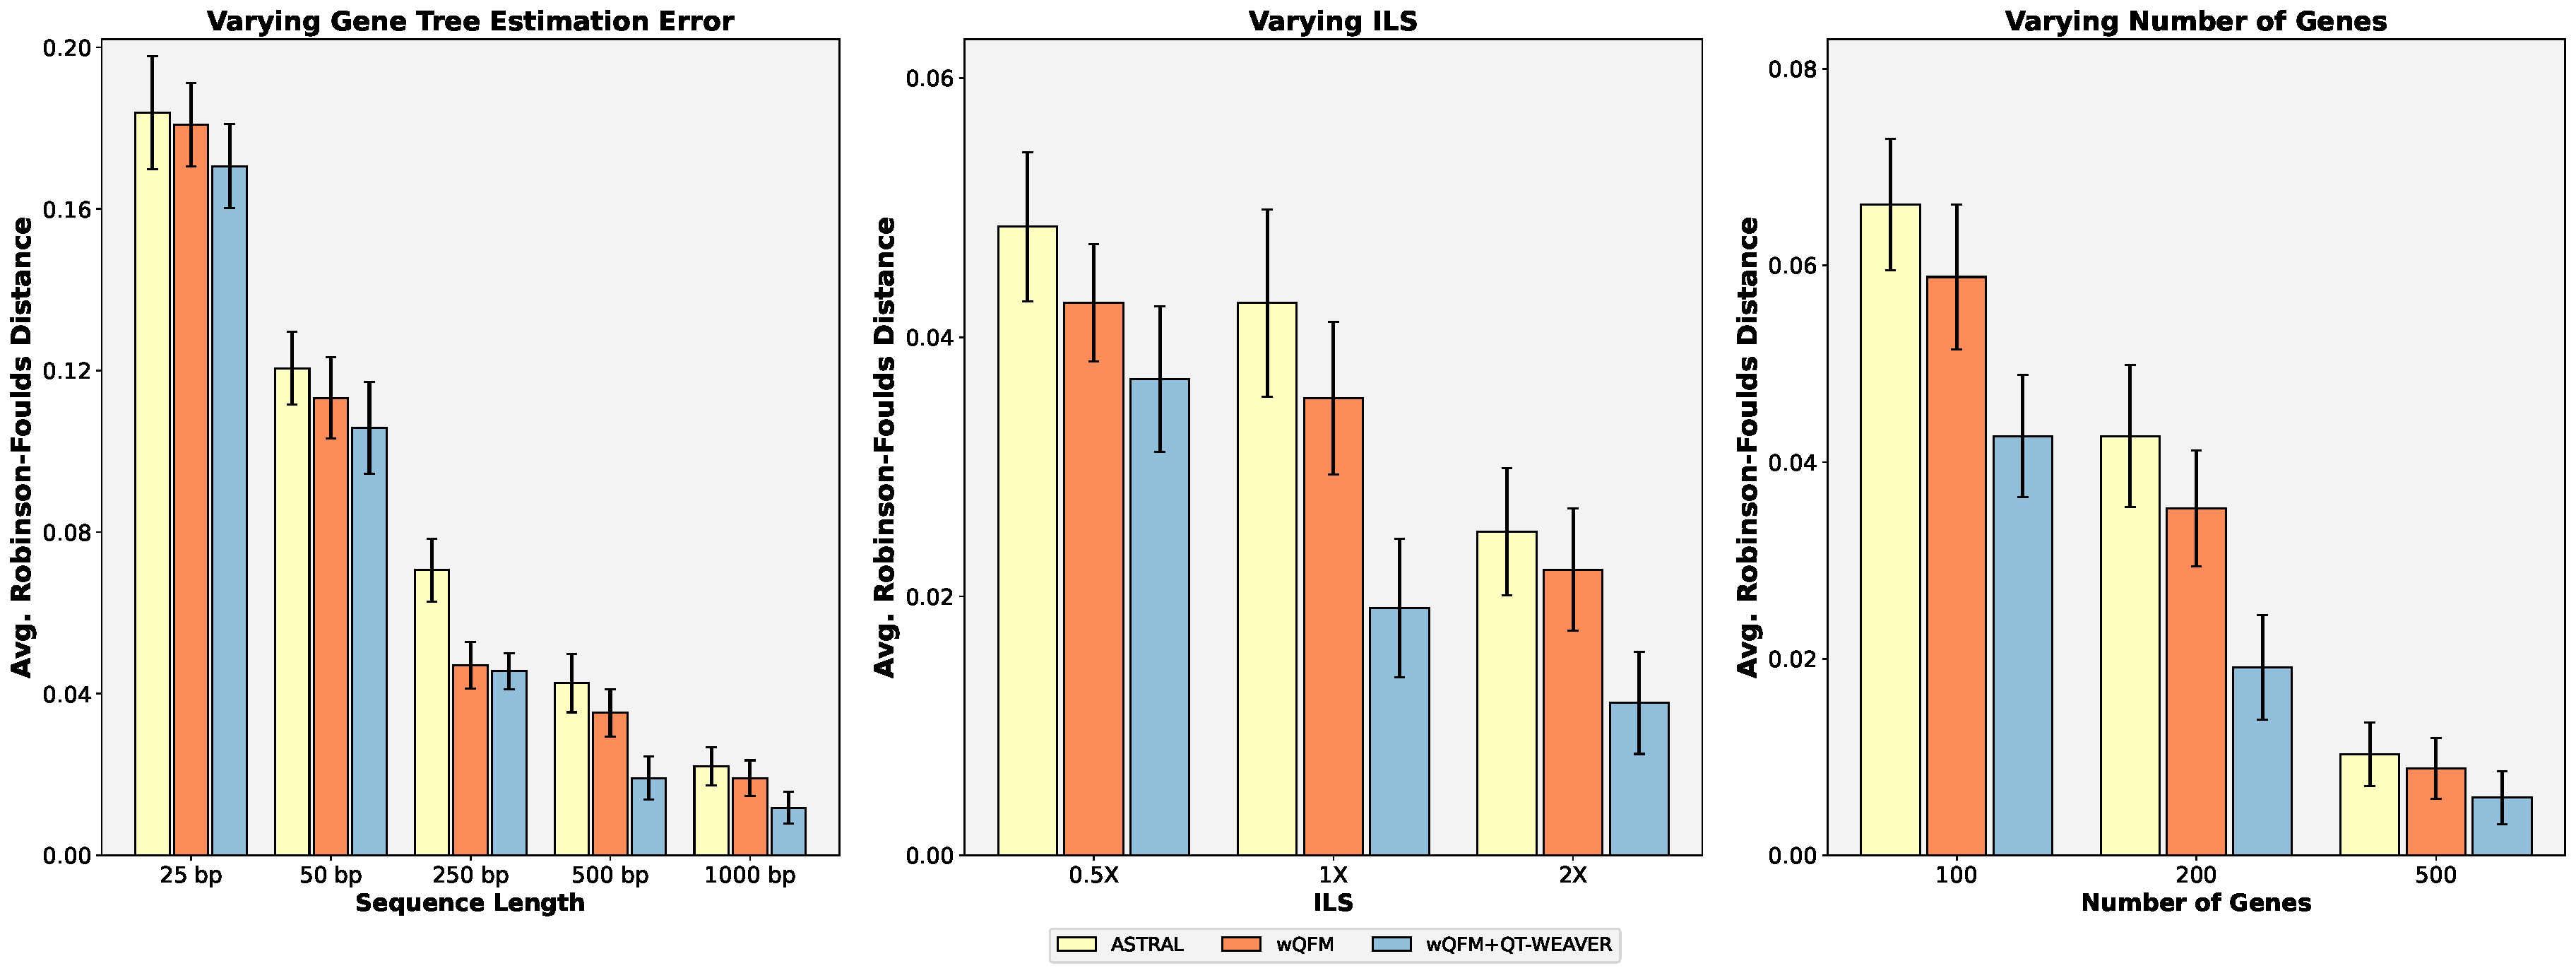
\includegraphics[width=\linewidth]{figures_new/2_37_methods.pdf}
    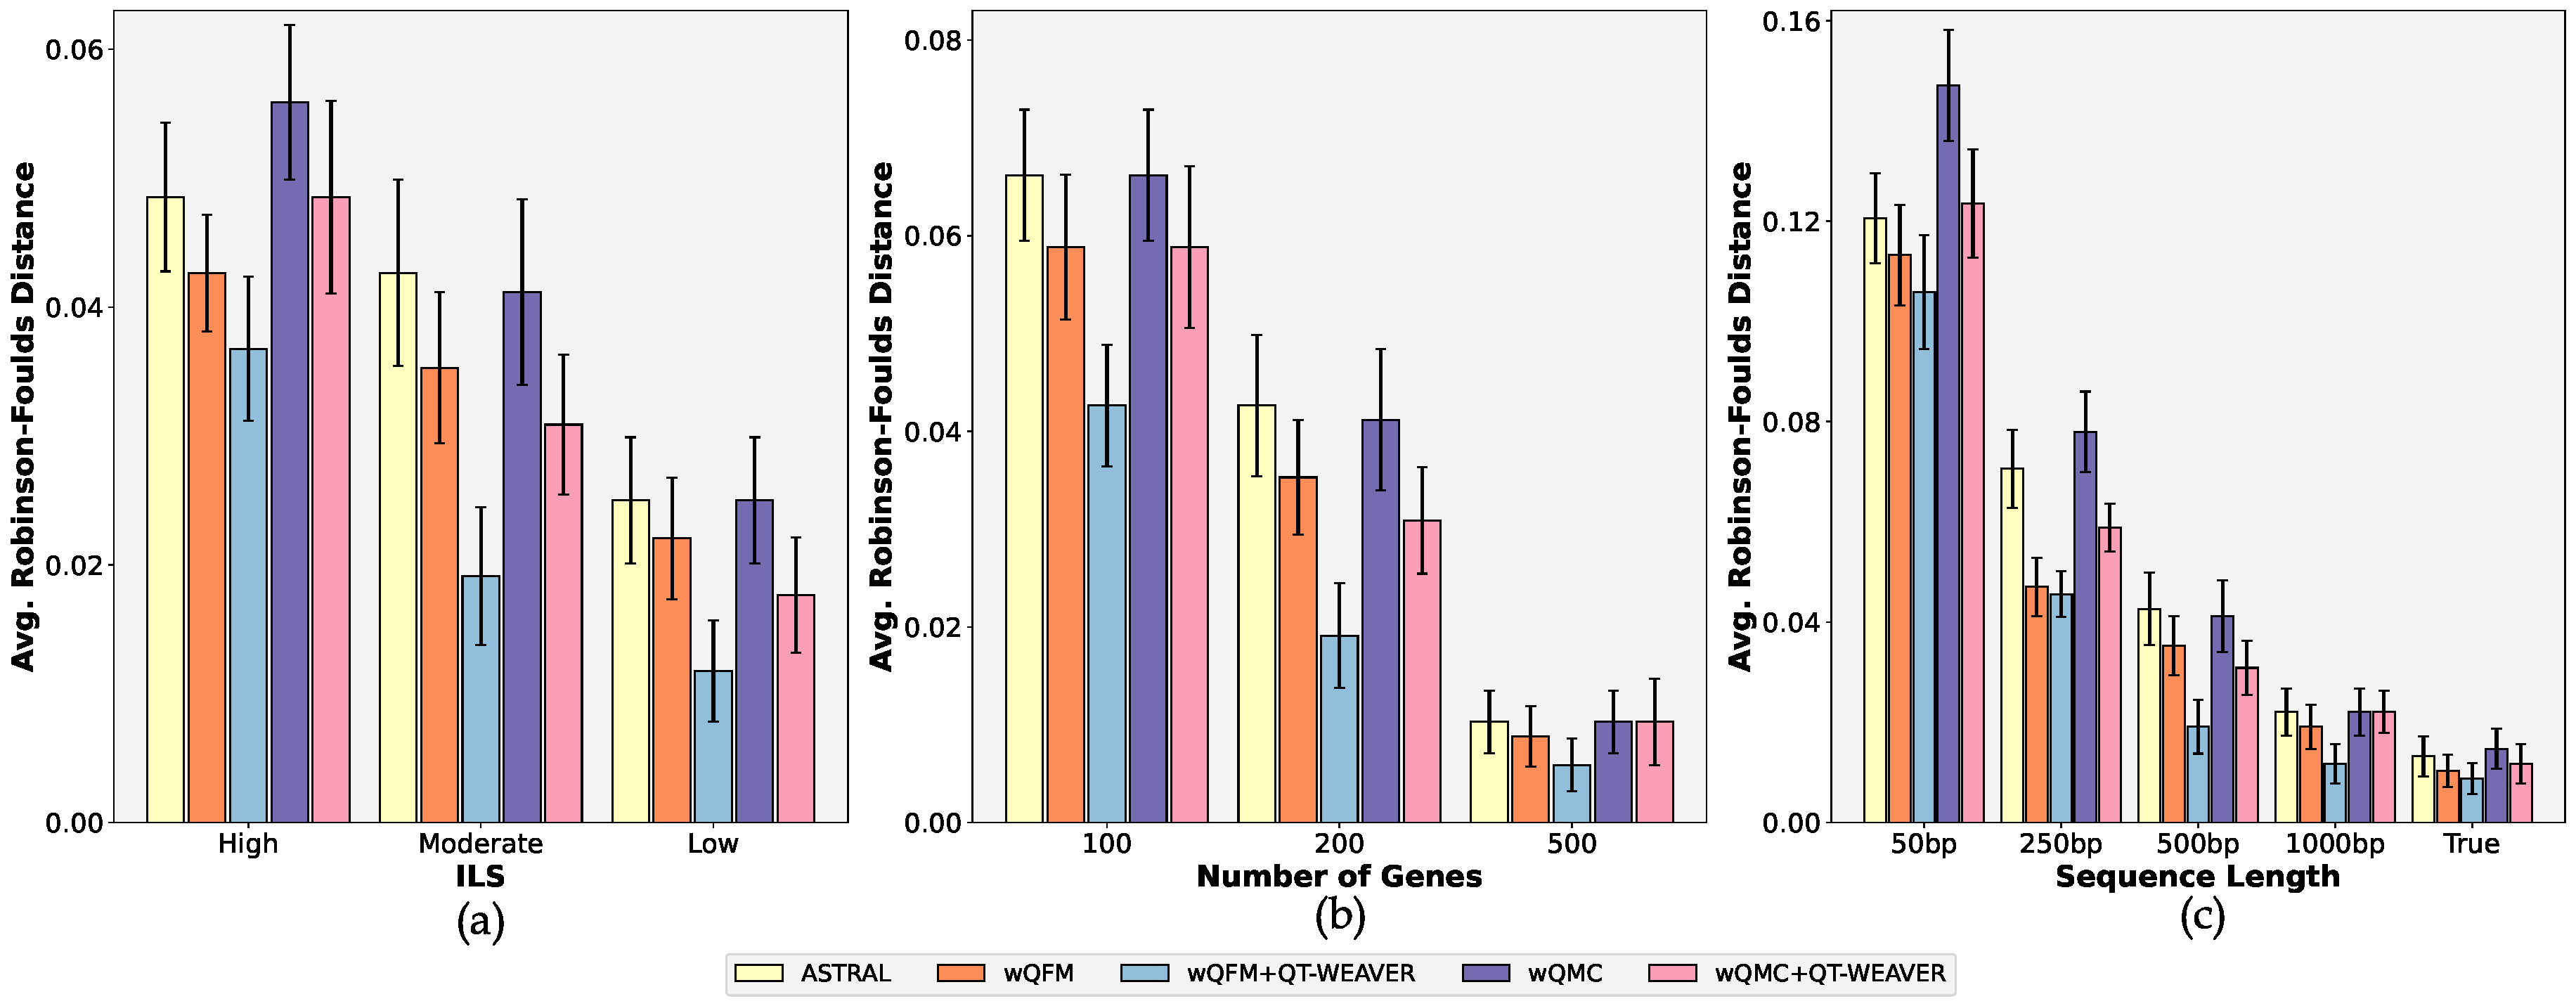
\includegraphics[width=\linewidth]{figures_new/9_37_methods_wqmc.pdf}
    \caption{\textbf{Results on 37-taxon dataset.} We show the average RF rates with standard errors over 20 replicates for the methods ASTRAL, wQFM (wQFM-uncorrected), wQFM+QT-WEAVER (wQFM-corrected), wQMC (wQMC-uncorrected), and wQMC+QT-WEAVER (wQMC-corrected). The settings in (a)-(c) are identical to the ones in Figure \ref{journal-fig:rf_37_taxon_methods} in the main paper. }
    \label{fig:rf_37_taxon_wqmc}
\end{figure}

\newpage

\subsection{Additional results on 15-taxon dataset}
\label{app:15-taxon}

% \begin{figure}[h!]
%     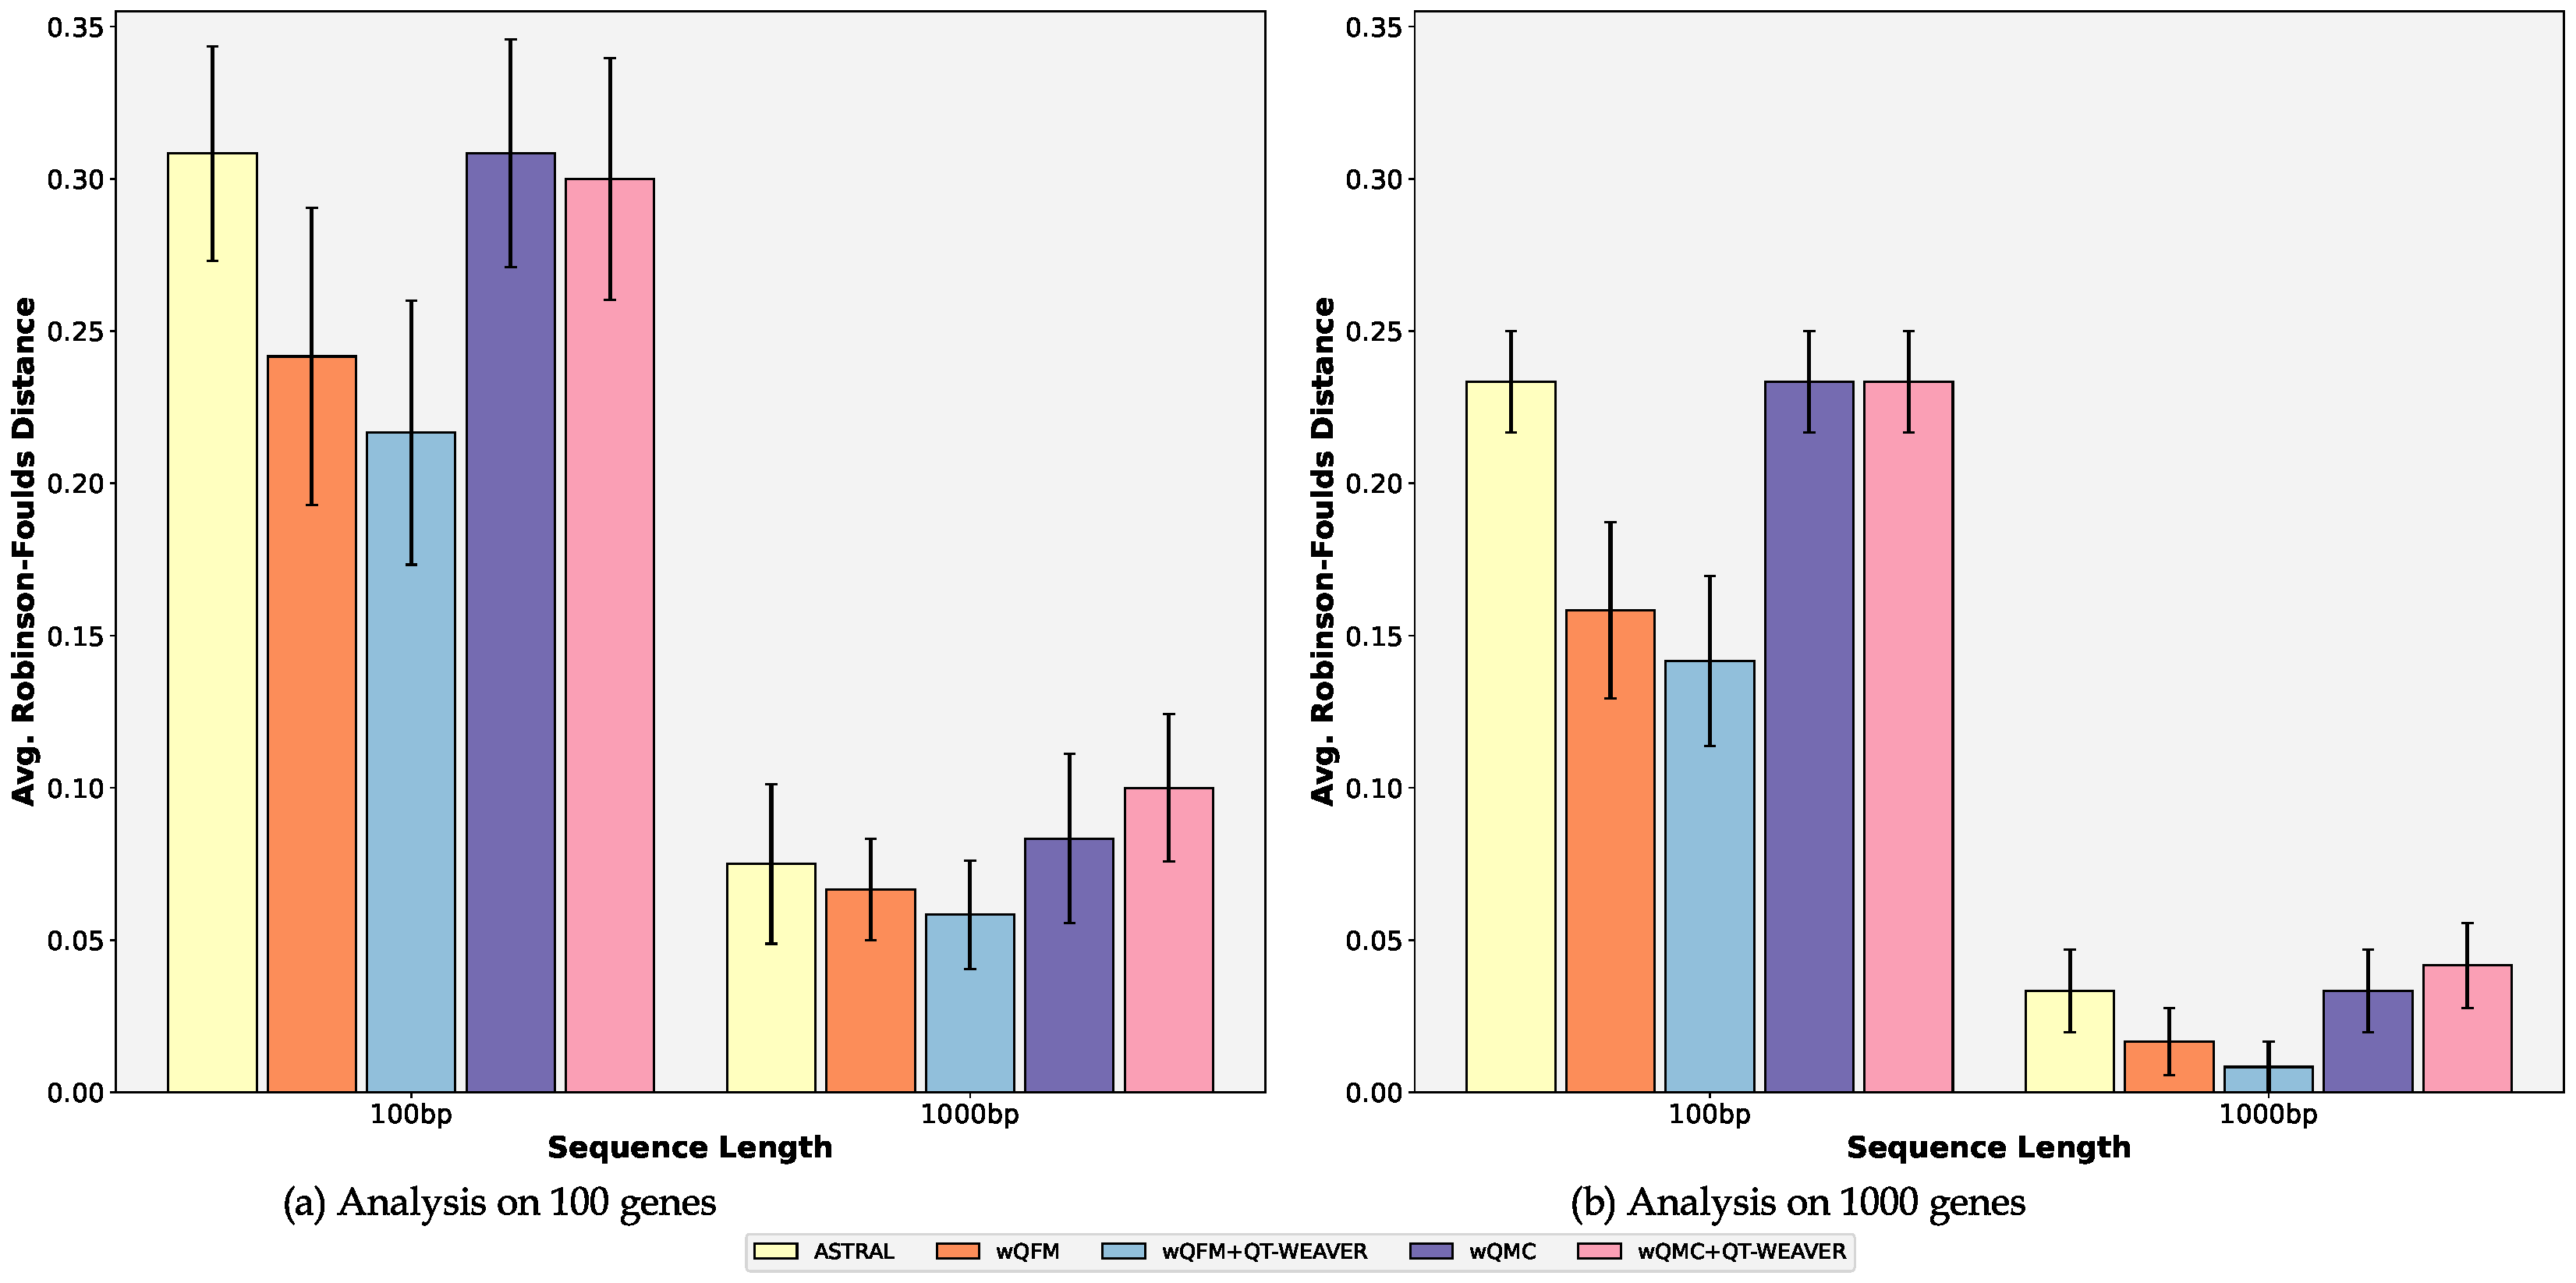
\includegraphics[width=\linewidth, height=0.5\linewidth]{figures_new/9_15_methods_wqmc.pdf}
%     \caption{\textbf{Results on 15-taxon dataset.} (a)-(b) We compare the average RF distance of ASTRAL, wQFM, wQFM+QT-WEAVER, wQMC, and wQMC+QT-WEAVER on varying model conditions. The settings are identical to the ones in Figure \ref{fig:rf_15_taxon_methods}.}
%     \label{fig:rf_15_taxon_methods_wqmc}
% \end{figure}


\begin{table}[h!]
    \centering
    % \small
    % \tiny
    \caption{The Jensen-Shannon divergence with respect to the true gene trees for different model conditions averaged over all replicates. The best-performing method (i.e., the least amount of divergence) for each model condition has been highlighted in bold.}
    % \bigskip
    \label{tab:15-divergence}

    \begin{tabular}{|c|C{3cm}|C{3cm}|}
        \hline
        \textbf{Model Condition} & \textbf{GTF} & \textbf{QT-WEAVER} \\
        \hline
        100gene-100bp & 0.115 & \textbf{0.103} \\
        \hline
        100gene-1000bp & \textbf{0.043} & 0.049 \\
        \hline
        1000gene-100bp & 0.101 & \textbf{0.087} \\
        \hline
        1000gene-1000bp & \textbf{0.031} & 0.037 \\
        \hline
    \end{tabular}
\end{table}

\begin{table}[h!]
    \centering
    % \small
    % \tiny
    \caption{Average quartet scores of estimated species trees and the true tree with respect to the estimated gene trees for the 15-taxon dataset. For wQFM+QT-WEAVER, we also report the quartet score with respect to the corrected estimated quartet distribution. The highest scores among the estimated trees have been italicized, and the scores closest to the true tree are shown in bold.}
    % \bigskip
    \label{tab:15-quartet-scores-estimated}
    \begin{tabular}{|C{2cm}|C{2.5cm}|C{2.5cm}|C{2.5cm}|C{2.5cm}|C{2.5cm}|}
        \hline
        \textbf{Model Condition} & \textbf{ASTRAL} & \textbf{wQFM} & \textbf{wQFM+QT-WEAVER (Original Distribution)} & \textbf{wQFM+QT-WEAVER (Corrected Distribution)} & \textbf{True Tree} \\
        \hline \hline
        100gene-100bp & 69934 & \textbf{69777} & 69792 & \textit{73598} & 69307 \\
        \hline
        100gene-1000bp & 82167 & 82129 & \textbf{82125} & \textit{87562} & 82099 \\
        \hline
        1000gene-100bp & 693656 & 692949 & \textbf{692664} & \textit{727712} & 690268 \\
        \hline
        1000gene-1000bp & 818022 & 817994 & \textbf{817953} & \textit{869904} & 817937 \\
        \hline
    \end{tabular}
\end{table}

\begin{table}[h!]
    \centering
    % \small
    % \tiny
    \caption{Average quartet scores of estimated species trees and the true tree with respect to the true gene trees for the 15-taxon dataset. The highest scores among the estimated trees have been italicized, and the scores closest to the true tree are shown in bold.}
    % \bigskip
    \label{tab:15-quartet-scores-true}
    \begin{tabular}{|C{2.3cm}|C{3cm}|C{3cm}|C{3cm}|C{3cm}|}
        \hline
        \textbf{Model Condition} & \textbf{ASTRAL} & \textbf{wQFM} & \textbf{wQFM+QT-WEAVER} & \textbf{True  Tree} \\
        \hline \hline
        100gene-100bp & 82159 & 82708 & \textbf{\textit{83078}} & 84635 \\
        \hline
        100gene-1000bp & 84345 & 84437 & \textbf{\textit{84444}} & 84635 \\
        \hline
        1000gene-100bp & 827970 & 834890 & \textbf{\textit{836349}} & 844184 \\
        \hline
        1000gene-1000bp & 843363 & 843792 & \textbf{\textit{843973}} & 844184 \\
        \hline
    \end{tabular}
\end{table}

%On the other hand, maximizing the quartet scores with respect to the estimated gene trees may not guarantee more accuracy in the presence of gene tree estimation errors and limited number of genes. The true tree having the lowest quartet scores across all model conditions supports this claim (Table \ref{tab:15-quartet-scores-estimated}). ASTRAL attains the highest quartet scores, which is furthest from the true tree, suggesting that it is ``overshooting" the quartet scores as it returns the least accurate tree among the three methods. Clearly, the wQFM+QT-WEAVER species trees, when compared to the original estimated distribution, are suffering from this ``overshooting" issue the least, which results in the best trees. Interestingly, when we consider the ``corrected" estimated distribution, the quartet scores of wQFM+QT-WEAVER are by far the highest, indicating that the corrected distribution was able to shed much of the limitations caused by gene tree estimation error and a limited number of genes. Hence, the corrected distribution is a more reliable representation of the true distribution.

\clearpage

\subsection{Additional results on 48-taxon dataset}
\label{app:48-taxon}
\begin{table}[h!]
    \centering
    % \small
    % \tiny
    \caption{The Jensen-Shannon divergence with respect to the true gene trees for different model conditions averaged over all replicates. The best-performing method (i.e., the least amount of divergence) for each model condition has been highlighted in bold.}
    % \bigskip
    \label{tab:48-divergence}

    \begin{tabular}{|c|C{3cm}|C{3cm}|}
        \hline
        \textbf{Model Condition} & \textbf{GTF} & \textbf{QT-WEAVER} \\
        \hline
        0.5X-1000-500 & 0.053 & \textbf{0.05} \\
        \hline
        1X-50-500 & 0.119 & \textbf{0.115} \\
        \hline
        1X-100-500 & 0.104 & \textbf{0.1} \\
        \hline
        1X-200-500 & 0.095 & \textbf{0.09} \\
        \hline
        1X-500-500 & 0.088 & \textbf{0.084} \\
        \hline
        1X-1000-500 & 0.086 & \textbf{0.082} \\
        \hline
        2X-1000-500 & 0.129 & \textbf{0.125} \\
        \hline
    \end{tabular}
\end{table}

\begin{table}[h!]
    \centering
    % \small
    % \tiny
    \caption{Average quartet scores of estimated species trees and the true tree with respect to the estimated gene trees for the 48-taxon dataset. For wQFM+QT-WEAVER, we also report the quartet score with respect to the corrected estimated quartet distribution. The highest scores among the estimated trees have been italicized, and the scores closest to the true tree are shown in bold.}
    % \bigskip
    \label{tab:48-quartet-scores-estimated}
    \begin{tabular}{|C{2cm}|C{2.5cm}|C{2.5cm}|C{2.5cm}|C{2.5cm}|C{2.5cm}|}
        \hline
        \textbf{Model Condition} & \textbf{ASTRAL} & \textbf{wQFM} & \textbf{wQFM+QT-WEAVER (Original Distribution)} & \textbf{wQFM+QT-WEAVER (Corrected Distribution)} & \textbf{True Tree} \\
        \hline \hline
        0.5X-1000-500 & 110583149 & 110590454 & \textbf{110571852} & \textit{111644682} & 110526513 \\
        \hline
        1X-50-500 & 6204884 & 6191081 & \textbf{6188251} & \textit{6301099} & 6109255 \\
        \hline
        1X-100-500 & 12349311 & \textbf{12324222} & 12328065 & \textit{12509069} & 12250259 \\
        \hline
        1X-200-500 & 24632824 & 24606334 & \textbf{24602225} & \textit{24885625} & 24553381 \\
        \hline
        1X-500-500 & \textbf{3106420} & 3101726 & 3107694 & \textit{3134254} & 3104926 \\
        \hline
        1X-1000-500 & 123024938 & 122994498 & \textbf{122983971} & \textit{124026278} & 122945091 \\
        \hline
        2X-1000-500 & 131631394 & 131619670 & \textbf{131603624} & \textit{132583373} & 131567523 \\
        \hline
    \end{tabular}
\end{table}

\begin{table}[h!]
    \centering
    % \small
    % \tiny
    \caption{Average quartet scores of estimated species trees and the true tree with respect to the true gene trees for the 48-taxon dataset. The highest scores among the estimated trees have been italicized, and the scores closest to the true tree are shown in bold.}
    % \bigskip
    \label{tab:48-quartet-scores-true}
    \begin{tabular}{|C{2.3cm}|C{3cm}|C{3cm}|C{3cm}|C{3cm}|}
        \hline
        \textbf{Model Condition} & \textbf{ASTRAL} & \textbf{wQFM} & \textbf{wQFM+QT-WEAVER} & \textbf{True  Tree} \\
        \hline \hline
        0.5X-1000-500 & 119513732 & 119525755 & \textbf{\textit{119540365}} & 119669367 \\
        \hline
        1X-50-500 & 6746768 & 6743642 & \textbf{\textit{6753059}} & 6789683 \\
        \hline
        1X-100-500 & 13506775 & 13506470 & \textbf{\textit{13513183}} & 13610325 \\
        \hline
        1X-200-500 & \textbf{\textit{27093454}} & 27091736 & 27086810 & 27229537 \\
        \hline
        1X-500-500 & \textbf{\textit{3418291}} & 3415138 & 3417996 & 3424968 \\
        \hline
        1X-1000-500 & 135991280 & \textbf{\textit{136016624}} & 136009169 & 136107790 \\
        \hline
        2X-1000-500 & \textbf{\textit{148393885}} & 148377461 & 148321043 & 148466576 \\
        \hline
    \end{tabular}
\end{table}

% \newpage
\clearpage

% \subsection{Additional results on iterative corrections using QT-WEAVER}
% \label{app:iterations}

% We investigated how the Jensen-Shannon divergence evolves across iterations (see Figure \ref{fig:rf_15_taxon_iterative_2}(a) in Appendix \ref{app:iterations}). Initially, the divergence decreases during the first one or two iterations but then begins to increase. This occurs because, for the three alternative quartet topologies ($ab|cd, ac|bd, ad|bc$) on four taxa, QT-WEAVER tends to prioritize the quartet topology it identifies as ``correct'' --the one with the least conflict score--by increasing its weight while reducing the weights of the alternative topologies.  Thus, with successive iterations, the weight of the ``correct'' quartet topology continues to rise (toward 100\%) while the weights of the other two alternatives keep decreasing (toward 0\%). Thus, this overestimation of the weight of the ``correct'' quartets and the underestimation of the weights of the ``incorrect'' ones lead the adjusted distribution to diverge from the true weighted distribution. Despite this divergence, the iterative adjustments may still guide the tree search algorithm toward more accurate trees (up to a certain point) by emphasizing and amalgamating the quartets with higher weights, as evidenced by the gradual decrease in the RF rates up to 10-15 iterations. For the same reason, when examining the quartet scores of wQFM+QT-WEAVER with respect to the corresponding corrected quartet distribution (instead of the original quartet distribution), the scores continue to increase, approaching nearly 100\% (see Figure \ref{fig:rf_15_taxon_iterative_2}(b) in Appendix \ref{app:iterations}). This occurs because, in the corrected distribution, the weights of the quartets present in the estimated species trees steadily rise, resulting in higher quartet scores for the estimated trees.


% \begin{figure}[h!]
%     \centering % <-- added
%     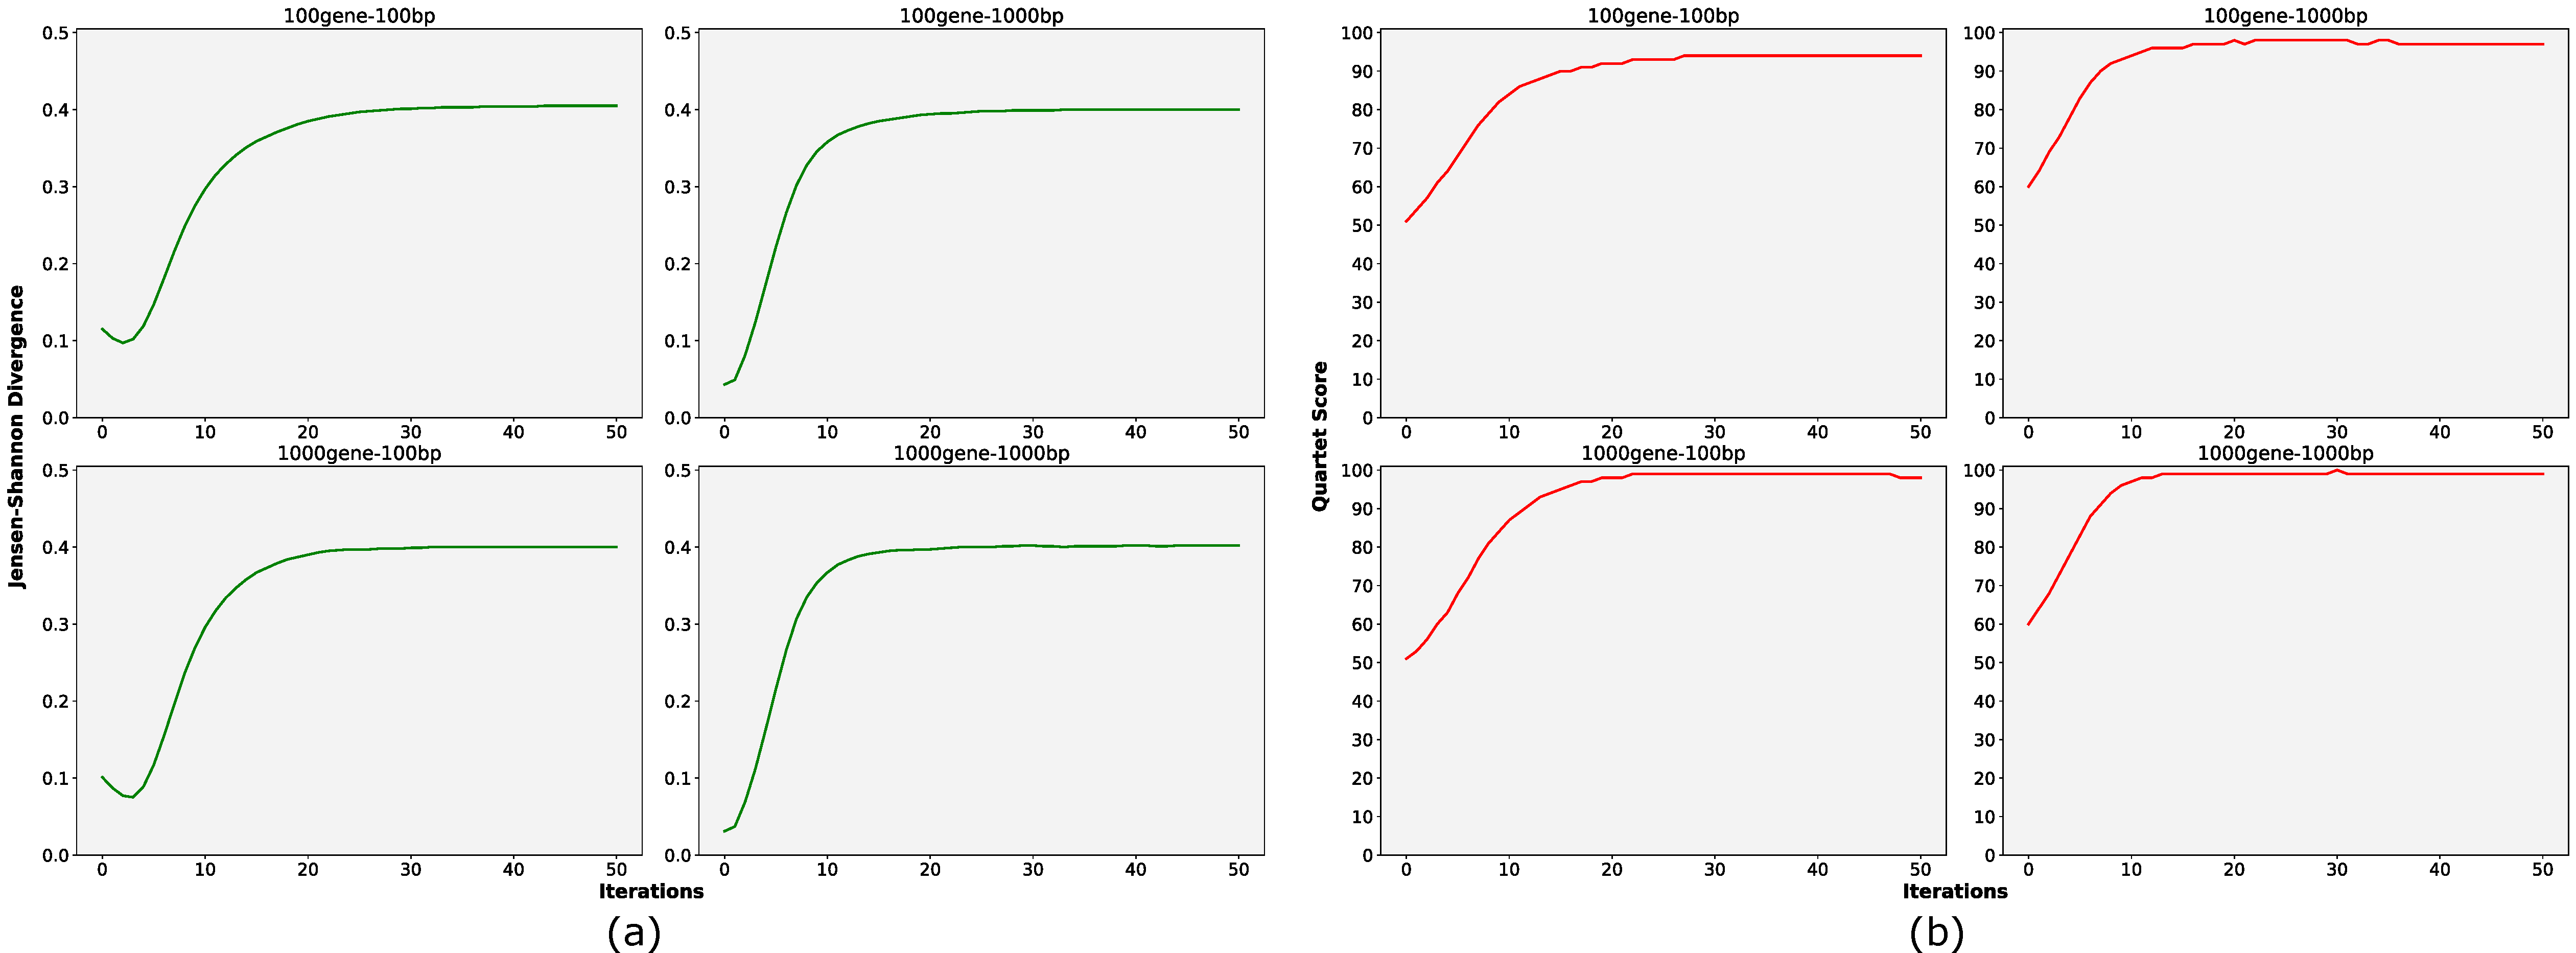
\includegraphics[width=\linewidth]{figures_new/15_iterative_2.pdf}
%     \caption{\textbf{Results iterative corrections on 15-taxon dataset.} We show the changes in (a) Jensen-Shannon divergence with respect to the true quartet distribution and (b) the quartet score of the estimated species tree with respect to its corresponding corrected quartet distribution over 50 iterations. 
%     }
%     \label{fig:rf_15_taxon_iterative_2}
% \end{figure}


% \subsection{Running time}
% \label{app:running-time}
% \begin{table}[htbp]
% \caption{Running time of QT-GILD for one epoch on different dataset.}
% \label{table.running time}
% \centering
% \begin{tabular}{c  c c } 
%  \toprule
%  Dataset &  \# Genes & Running time (seconds)  \\  [0.5ex]
%  \hline\hline
%  15-taxon & 100 & 25\times10^{-3} - 26\times10^{-3} \\
%  15-taxon & 1000 & 750\times10^{-3} - 800\times10^{-3} \\ \midrule
%  37-taxon & 100 & 1 $-$ 1.5\\
%  37-taxon & 200 & 2 $-$ 3\\
%  37-taxon & 400 & 5 $-$ 6\\ \midrule
%  Angiosperm (46-taxon) & 310 & 10 $-$ 11\\
%  \bottomrule
 
% \end{tabular}
% \end{table}

% \newpage

% \section{Analysis of Avian Biological Dataset}
% \label{app:avian-biological}


\bibliographystyle{unsrt}
% \bibliography{References}
\bibliographystyle{IEEEtran}
\bibliography{references.bib} % NEED TO CHANGE to references.bib

\end{document}